\documentclass[10pt]{article}

%%%%%%%%%%%%%%%%%%%%%%%%%%%%%%%%%%%%%%%%%%%%%%%%%%%%%%%%%%%%%%%%%%%%%%%%%%%%%%%%
% LaTeX Imports
%%%%%%%%%%%%%%%%%%%%%%%%%%%%%%%%%%%%%%%%%%%%%%%%%%%%%%%%%%%%%%%%%%%%%%%%%%%%%%%%
\usepackage{amsfonts}                                                   % Math fonts
\usepackage{amsmath}                                                    % Math formatting
\usepackage{amssymb}                                                    % Math formatting
\usepackage{amsthm}                                                     % Math Theorems
\usepackage{arydshln}                                                   % Dashed hlines
\usepackage{attachfile}                                                 % AttachFiles
\usepackage{cancel}                                                     % Cancelled math
\usepackage{caption}                                                    % Figure captioning
\usepackage{color}                                                      % Nice Colors
\input{./lib/dragon.inp}                                                % Tikz dragon curve
\usepackage[ampersand]{easylist}                                        % Easy lists
\usepackage{fancyhdr}                                                   % Fancy Header
\usepackage[T1]{fontenc}                                                % Specific font-encoding
%\usepackage[margin=1in, marginparwidth=2cm, marginparsep=2cm]{geometry} % Margins
\usepackage{graphicx}                                                   % Include images
\usepackage{hyperref}                                                   % Referencing
\usepackage[none]{hyphenat}                                             % Don't allow hyphenation
\usepackage{lipsum}                                                     % Lorem Ipsum Dummy Text
\usepackage{listings}                                                   % Code display
\usepackage{marginnote}                                                 % Notes in the margin
\usepackage{microtype}                                                  % Niceness
\usepackage{lib/minted}                                                 % Code display
\usepackage{multirow}                                                   % Multirow tables
\usepackage{pdfpages}                                                   % Include pdfs
\usepackage{pgfplots}                                                   % Create Pictures
\usepackage{rotating}                                                   % Figure rotation
\usepackage{setspace}                                                   % Allow double spacing
\usepackage{subcaption}                                                 % Figure captioning
\usepackage{tikz}                                                       % Create Pictures
\usepackage{tocloft}                                                    % List of Equations
%%%%%%%%%%%%%%%%%%%%%%%%%%%%%%%%%%%%%%%%%%%%%%%%%%%%%%%%%%%%%%%%%%%%%%%%%%%%%%%%
% Package Setup
%%%%%%%%%%%%%%%%%%%%%%%%%%%%%%%%%%%%%%%%%%%%%%%%%%%%%%%%%%%%%%%%%%%%%%%%%%%%%%%%
\hypersetup{%                                                           % Setup linking
    colorlinks=true,
    linkcolor=black,
    citecolor=black,
    filecolor=black,
    urlcolor=black,
}
\RequirePackage[l2tabu, orthodox]{nag}                                  % Nag about bad syntax
\renewcommand*\thesection{\arabic{section} }                             % Reset numbering
\renewcommand{\theFancyVerbLine}{ {\arabic{FancyVerbLine} } }              % Needed for code display
\renewcommand{\footrulewidth}{0.4pt}                                    % Footer hline
\setcounter{secnumdepth}{3}                                             % Include subsubsections in numbering
\setcounter{tocdepth}{3}                                                % Include subsubsections in toc
%%%%%%%%%%%%%%%%%%%%%%%%%%%%%%%%%%%%%%%%%%%%%%%%%%%%%%%%%%%%%%%%%%%%%%%%%%%%%%%%
% Custom commands
%%%%%%%%%%%%%%%%%%%%%%%%%%%%%%%%%%%%%%%%%%%%%%%%%%%%%%%%%%%%%%%%%%%%%%%%%%%%%%%%
\newcommand{\nvec}[1]{\left\langle #1 \right\rangle}                    %  Easy to use vector
\newcommand{\ma}[0]{\mathbf{A} }                                         %  Easy to use vector
\newcommand{\mb}[0]{\mathbf{B} }                                         %  Easy to use vector
\newcommand{\abs}[1]{\left\lvert #1 \right\rvert}                       %  Easy to use abs
\newcommand{\pren}[1]{\left( #1 \right)}                                %  Big parens
\let\oldvec\vec
\renewcommand{\vec}[1]{\oldvec{\mathbf{#1} } }                            %  Vector Styling
\newtheorem{thm}{Theorem}                                               %  Define the theorem name
\newtheorem{definition}{Definition}                                     %  Define the definition name
\definecolor{bg}{rgb}{0.95,0.95,0.95}
\newcommand{\java}[4]{\vspace{10pt}\inputminted[firstline=#2,
                                 lastline=#3,
                                 firstnumber=#2,
                                 gobble=#4,
                                 frame=single,
                                 label=#1,
                                 bgcolor=bg,
                                 linenos]{java}{#1} }
\newcommand{\python}[4]{\vspace{10pt}\inputminted[firstline=#2,
                                 lastline=#3,
                                 firstnumber=#2,
                                 gobble=#4,
                                 frame=single,
                                 label=#1,
                                 bgcolor=bg,
                                 linenos]{python}{#1} }
\newcommand{\js}[4]{\vspace{10pt}\inputminted[firstline=#2,
                                 lastline=#3,
                                 firstnumber=#2,
                                 gobble=#4,
                                 frame=single,
                                 label=#1,
                                 bgcolor=bg,
                                 linenos]{js}{#1} }
%%%%%%%%%%%%%%%%%%%%%%%%%%%%%%%%%%%%%%%%%%%%%%%%%%%%%%%%%%%%%%%%%%%%%%%%%%%%%%%%
% Beginning of document items - headers, title, toc, etc...
%%%%%%%%%%%%%%%%%%%%%%%%%%%%%%%%%%%%%%%%%%%%%%%%%%%%%%%%%%%%%%%%%%%%%%%%%%%%%%%%
\pagestyle{fancy}                                                       %  Establishes that the headers will be defined
\fancyhead[LE,LO]{Computer Systems Notes}                                  %  Adds header to left
\fancyhead[RE,RO]{Zoe Farmer}                                       %  Adds header to right
\cfoot{ \thepage }
\lfoot{CSCI 2400}
\rfoot{Han}
\title{Computer Systems Notes}
\author{Zoe Farmer}

%%%%%%%%%%%%%%%%%%%%%%%%%%%%%%%%%%%%%%%%%%%%%%%%%%%%%%%%%%%%%%%%%%%%%%%%%%%%%%%%
% Beginning of document items - headers, title, toc, etc...
%%%%%%%%%%%%%%%%%%%%%%%%%%%%%%%%%%%%%%%%%%%%%%%%%%%%%%%%%%%%%%%%%%%%%%%%%%%%%%%%
\pagestyle{fancy}                                                       %  Establishes that the headers will be defined
\fancyhead[LE,LO]{Homework 5}                                  %  Adds header to left
\fancyhead[RE,RO]{Zoe Farmer}                                       %  Adds header to right
\cfoot{\mlptikz[size=0.25in, text=on, textposx=0, textposy=0, textvalue=\thepage, textscale=0.75in]{applejack}}
\lfoot{APPM 3570}
\rfoot{Kleiber}
\title{Homework 5}
\date{Kleiber}
\author{Zoe Farmer - 101446930}
%%%%%%%%%%%%%%%%%%%%%%%%%%%%%%%%%%%%%%%%%%%%%%%%%%%%%%%%%%%%%%%%%%%%%%%%%%%%%%%%
% Beginning of document items - headers, title, toc, etc...
%%%%%%%%%%%%%%%%%%%%%%%%%%%%%%%%%%%%%%%%%%%%%%%%%%%%%%%%%%%%%%%%%%%%%%%%%%%%%%%%
\begin{document}

\maketitle

\begin{table}[!ht]
    \centering
    \scalebox{1.5}{%
    \begin{tabular}{|l|l|l|l||l|}
        \hline
        1 & 2 & 3 & 4 & T\\
        \hline
        & & & &\\
        \hline
    \end{tabular}
    }
\end{table}

\begin{easylist}[enumerate]
    \ListProperties(Hide1=50, Space1=1cm)
    @ \textit{Chapter 4, \#22 --} Suppose that two teams play a series of games that ends when one of them has won $i$
    games. Suppose that each game played is, independently, won by team $A$ with probability $p$. Find the expected
    number of games that are played when\footnote{Also, show in both cases that this number is maximized when
    $p=\frac{1}{2}$.}
    @@ $i = 2$
    @@@ If we let $P(B) = q = 1 - p$ then there are six different ways for the games to go with corresponding
    probabilities.

        \[ \begin{aligned}
            \{ AA,& ABA,& ABB,& BB,& BAB,& BAA \}\\
            \{ p^2,& qp^2,& pq^2,& q^2,& pq^2,& qp^2\}
        \end{aligned} \]

    In order to find the expected number of games we use the formula

        \[ \sum_D x \cdot p(x) = 2 p^2 + 3qp^2 + 3pq^2 + 2q^2 + 3pq^2 + 3qp^2 = 2 + 2 p - 2 p^2 = 2p(1-p)+2 \]

    If we let $p=0.5$ we see this value is maximized at 2.5. Please see Figure~\ref{fig:1.1}.

    \begin{figure}[!ht]
        \centering
        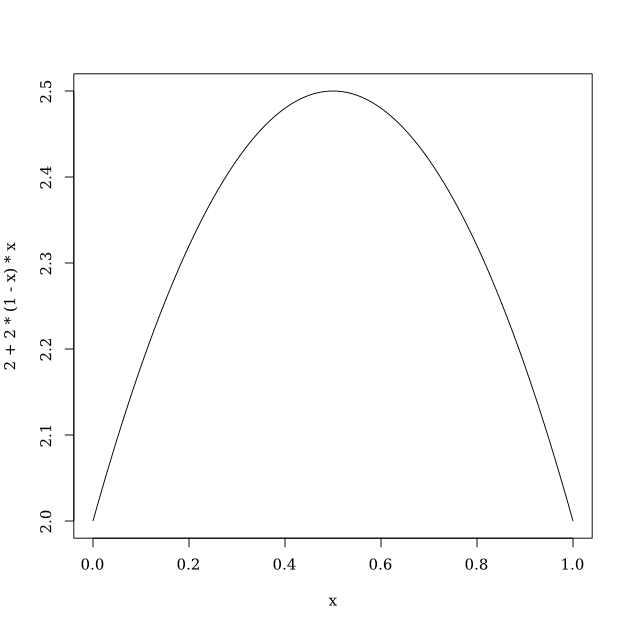
\includegraphics[scale=0.5]{./img/ps5_1.png}
        \caption{Plot of $p$ Variables}
        \label{fig:1.1}
    \end{figure}

    @@ $i = 3$
    @@@ We can use the same process and enumerate the ways for this to occur.\footnote{Some programming was used to
    quickly find the ways and probabilities}

        \[ \begin{aligned}
                &[(AABBB, p^2q^3), (AAA, p^3), (BBB, q^3), (ABBB, pq^3),\\
                &(AABBA, p^3q^2), (BBAB, pq^3), (ABABA, p^3q^2), (BAAA, qp^3),\\
                &(BABAB, p^2q^3), (ABBAB, p^2q^3), (BABB, pq^3), (BBAAB, p^2q^3),\\
                &(ABBAA, p^3q^2), (ABAA, qp^3), (BBAAA, p^3q^2), (AABA, qp^3),\\
                &(BAABB, p^2q^3), (BABAA, p^3q^2), (BAABA, p^3q^2), (ABABB, p^2q^3)]
        \end{aligned} \]

    Using the formula for expected value we find

        \[ \sum_D x \cdot p(x) = 3 (1 + p + p^2 - 4 p^3 + 2 p^4) \]

    And with $p=0.5$ we see that it is indeed a maximal value. Please see Figure~\ref{fig:1.2}.

    \begin{figure}[!ht]
        \centering
        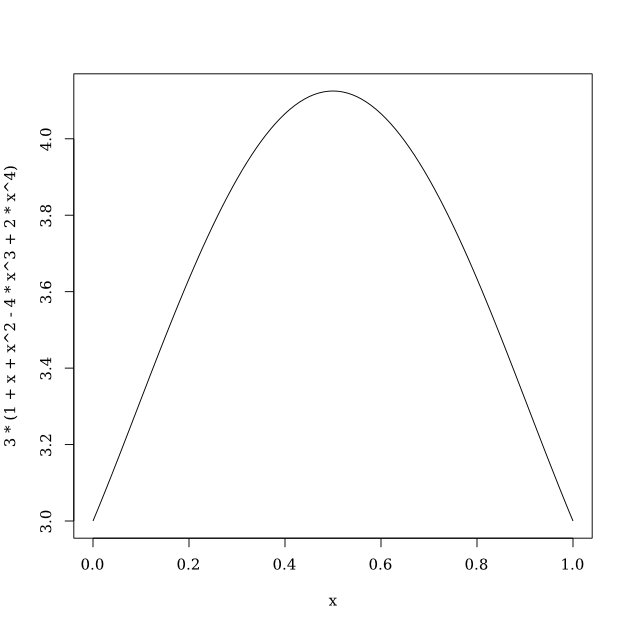
\includegraphics[scale=0.5]{./img/ps5_1_1.png}
        \caption{Plot of $p$ Variables}
        \label{fig:1.2}
    \end{figure}

    @ \textit{Chapter 4, \#28 --} A sample of 3 items is selected at random from a box containing 20 items of which 4
    are defective. Find the expected number of defective items in the sample.
    @@ There are $\binom{20}{3}$ ways to take 3 items from 20, and each has probability $\frac{4}{20} = 0.2$ of being
    defective. Letting $X$ be the number of defective items we have, we can determine the pmf.

        \[
            p(x) =
            \begin{cases}
                \frac{\binom{16}{3-x} \binom{4}{x}}{\binom{20}{3}} &\to x=\{0, 1, 2, 3\}\\
                0 &\to Otherwise
            \end{cases}
        \]

    We can now find the expected number of defective items to be

        \[
            \sum_{i=0}^3 x \cdot p(x) = 0 \cdot p(0) + 1 \cdot p(1) + 2 \cdot p(2) + 3 \cdot p(3) = \frac{3}{5} =
            \boxed{0.6}
        \]

    @ \textit{Chapter 4, \#30 --} A person tosses a fair coin until a tail appears for the first time. If the tail
    appears on the $n$th flip, the person wins $2^n$ dollars. Let $X$ denote the player's winnings. Show that $E[X] =
    +\infty$. This problem is known as the St. Petersburg paradox.
    @@ The probability that a tail appears on the $n$th flip means that there must be $n - 1$ heads and then a tail.
    This probability is given by

        \[ {\left( \frac{1}{2} \right)}^n \]

    With expected value of winnings given by

        \[ \sum_{i = 1}^{\infty} 2^n {\left( \frac{1}{2} \right)}^n = \sum_{i=1}^{\infty} 1 = \infty \]

    @ \textit{Chapter 4, \#36 --} Consider Problem 22 with $i = 2$. Find the variance of the number of games played,
    and show that this number is maximized when $p = \frac{1}{2}$.
    @@ The formula for Variance is

        \[ \begin{aligned}
            V(X) &=&  E(X^2) - {[E(X)]}^2 = 4 + 10p - 10p^2 - {(2p(1-p)+2)}^2\\
                 &=& 2 p (1 - 3 p + 4 p^2 - 2 p^3)
        \end{aligned} \]

        And there is an inflection point at $p=0.5$.

    @ \textit{Chapter 4, \#38 --} If $E[X] = 1$ and $\text{Var}(X) = 5$, find
    @@ $E[{(2 + X)}^2]$
        \[ E[{(2 + X)}^2] = E[X^2 + 4X + 4] = E[X^2] + 4 E[X] + 4 = V(x) + {[E(X)]}^2 + 8 = \boxed{14} \]
    @@ $\text{Var}(4 + 3X)$
        \[ \text{Var}(4 + 3X) = \text{Var}(3X) = 9 \text{Var}(X) = \boxed{45} \]

    @ \textit{Chapter 4, \#44 --} A satellite system consists of $n$ components and functions on any given day if at
    least $k$ of the $n$ components function on that day. On a rainy day each of the components independently functions
    with probability $p_1$, whereas on a dry day they each independently function with probability $p_2$. If the
    probability of rain tomorrow is $\alpha$, what is the probability that the satellite system will function?
    @@ Let $R$ be the event that it rains, and $F$ be the event that the system is functional. We know $P(R) = \alpha$,
    $P(F|R) = p_1$, and $P(F|R^c) = p_2$, and we're interested in $P(F)$.

        \[
            P(F) = P(F|R)P(R) + P(F|R^c)(1-P(R)) = p_1 \cdot \alpha + p_2 (1 - \alpha)
        \]

    @ System reliability: System reliability is concerned with how long a system will operate before it breaks down and
    repairs are required. In this problem the system is an electric power plant consisting of four generators. These
    generators operate simultaneously to generate power. We will assume that each generator operates independently of
    all the others.  Suppose the probability that a generator fails in the $k^{th}$ month is given by a geometric
    probability mass function with probability of failure equal to 0.1. Thus, its probability mass function is:

        \[
            p(k) =
            \begin{cases}
                \frac{1}{10} {\left( \frac{9}{10} \right)}^{k - 1} &\to k = 1, 2, \ldots\\
                0 &\to Otherwise
            \end{cases}
        \]

    @@ What is the probability that none of the four generators fails in the first month of use?
    @@@ If we take the case of $k=1$, we find the probability of generator failure to be

        \[ p(1) = \frac{1}{10} \]

        Therefore the probability that no generators fail is

        \[ {\left( \frac{9}{10} \right)}^4 = \frac{6561}{10000} = \boxed{0.6561} \]

    @@ Suppose there is only one generator. What is the probability that it doesn't fail in the first 12 months? (Hint:
    If it doesn't fail in the first 12 months, when does it fail?)
    @@@ We can find this with the cdf of $p(k)$, which is defined as
        \[ F(x) = \sum_{i = 1}^{x} p(i) = 1 - {\left( \frac{9}{10} \right)}^x \]
        We're interested in the likelihood that it fails after 12 months, which is
        \[
            1 - F(12) = \frac{282429536481}{1000000000000} = \boxed{0.28243}
        \]
    @@ Now, use part (b) to find the probability that three out of four generators will be working after 1 year. (Hint:
    There are 2 random variables in this problem. What are they? What are their distributions?)
    @@@ We know the probability of each generator lasting 12 months, $1 - F(12)$. Let $X$ be the random variable
    counting how many generators survive after 12 months, and $p = F(12)$. We can determine the pmf of $X$.

        \[
            p(X) =
            \begin{cases}
                \binom{4}{x} p^{4 - x} {(p^c)}^{x} &\to x = {0, 1, 2, 3, 4}\\
                0 &\to Otherwise
            \end{cases}
        \]

    And now simply find $p(3) = \boxed{0.0646631}$

    @ A lumber company has just taken delivery on a lot of 10,000 $2 \times 4$ boards. Suppose that 20\% of these boards
    are actually too green to be used in first-quality construction.
    @@ Two boards are selected at random, one after the other. Let $A = \{\text{the first board is green}\}$ and $B =
    \{\text{the second board is green}\}$. Compute $P(A)$, $P(B)$ and $P(AB)$. Are $A$ and $B$ independent?
    @@@ We know that any board taken at random has $P(A) = \frac{2000}{10000} = 0.2$ chance of being green. We also know
    that the second board has $P(B) = \frac{2000}{10000} = 0.2$. If we take the intersection of these two events
    we can determine whether or not they are independent.

        \[ P(AB) = P(B|A)P(A) = \frac{1999}{9999} \cdot \frac{2000}{10000} = 0.03998 \neq P(A)P(B) \]

    @@ Now consider two independent events $A$ and $B$ with $P(A) = P(B) = 0.2$, what is $P(AB)$?  How much difference
    is there between this answer and $P(AB)$ in part (a)? For purposes of calculating $P(AB)$, can we assume that $A$
    and $B$ of part (a) are independent to obtain essentially the correct probability?
    @@@ If these two events are independent, then $P(AB) = P(A)P(B) = 0.04$, which has difference from part (a) of
    $0.00002$. In this case, since the numbers are so large we could theoretically just assume that $A$ and $B$ are
    independent to come to an approximation of $P(AB)$.
    @@ Now suppose the lot consists of ten boards, of which two are green. Does the assumption of independence now yield
    approximately the correct answer for $P(AB)$? What is the critical difference between the situation here and that of
    part (a)? When do you think that an independence assumption would be valid in obtaining an approximately correct
    answer to $P(AB)$?
    @@@ If only two out of ten boards are green, we can no longer make the prior assumption. If they're independent then
    the probability remains $0.04$, but if they aren't it becomes $0.0222222$, which is vastly different. The critical
    difference between the two cases is the size of the problem. The larger problem has less error in an approximation.
    It's usually not a \textit{good} idea to assume that two events are independent in order to determine their union,
    however for sufficiently large values we can sometimes assume that fact.

\end{easylist}

\end{document}
